\subsection{Verslaggewing onderdeel}

Die verslaggewing onderdeel is verantwoordelik vir die generering van
verskillende verslae vir administratiewe doeleindes, insluitend finansiële
verslae, bestellingstatistieke, gebruikersaktiwiteite, en stelselprestasie.
Dit ondersteun beide real-time en geskeduleerde verslaggenerering.

\begin{figure}[H]
    \centering
    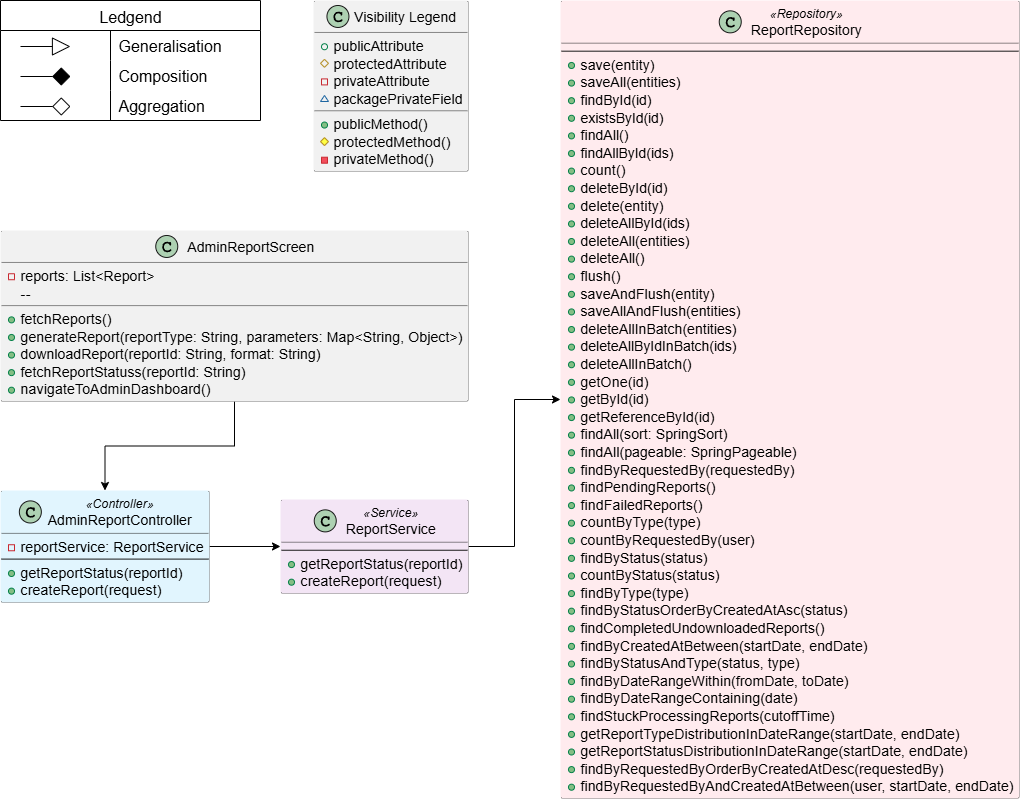
\includegraphics[width=\textwidth]{figures/class_diagrams/report-subsystem.png}
    \caption{Verslaggewing onderdeel klasdiagram}
    \label{fig:report_subsystem_class_diagram}
\end{figure}

Hier volg die CRC kaarte vir die belangrikste klasse in hierdie
onderdeel.

\vspace{1em}
\textbf{AdminReportScreen} bied administrateurs toegang tot verskillende verslag tipes, versoek generering, monitor status en laai verslae af.
\begin{table}[H]\centering\begin{tabular}{|p{0.4\textwidth}|p{0.4\textwidth}|}
    \hline
    \multicolumn{2}{|c|}{\textbf{AdminReportScreen}} \\
    \hline
    \textbf{Verantwoordelikhede} & \textbf{Medewerkers} \\
    \hline
    Wys beskikbare verslag tipes \newline
    Versoek verslag generering met parameters \newline
    Monitor verslag generering status \newline
    Laai verslae af in verskillende formate
    &
    AdminReportController \\
    \hline
\end{tabular}
\caption{CRC vir AdminReportScreen}
\label{tab:crc_admin_report_screen}
\end{table}

\vspace{1em}
\textbf{AdminReportController} hanteer verslagversoeke, inisieer generering, verskaf statusupdates en hanteer aflaai.
\begin{table}[H]\centering\begin{tabular}{|p{0.4\textwidth}|p{0.4\textwidth}|}
    \hline
    \multicolumn{2}{|c|}{\textbf{AdminReportController}} \\
    \hline
    \textbf{Verantwoordelikhede} & \textbf{Medewerkers} \\
    \hline
    Hanteer verslag versoeke van administrateurs \newline
    Inisieer verslag generering prosesse \newline
    Verskaf verslag status updates \newline
    Hanteer verslag aflaai versoeke
    &
    ReportService \\
    \hline
\end{tabular}
\caption{CRC vir AdminReportController}
\label{tab:crc_admin_report_controller}
\end{table}

\vspace{1em}
\textbf{ReportService} genereer verskillende tipes verslae, bestuur parameters en filters, hanteer formaatkonversies en monitor status.
\begin{table}[H]\centering\begin{tabular}{|p{0.4\textwidth}|p{0.4\textwidth}|}
    \hline
    \multicolumn{2}{|c|}{\textbf{ReportService}} \\
    \hline
    \textbf{Verantwoordelikhede} & \textbf{Medewerkers} \\
    \hline
    Genereer verskillende tipes verslae \newline
    Bestuur verslag parameters en filters \newline
    Hanteer verslag formaat konversies \newline
    Monitor en raporteer verslag status \newline
    Stoor en verkry gegenereerde verslae
    &
    ReportRepository \\
    \hline
\end{tabular}
\caption{CRC vir ReportService}
\label{tab:crc_report_service}
\end{table}

